\documentclass[journal]{IEEEtran}

\usepackage{hyperref}
\usepackage{graphicx} % Required for inserting images

\title{Ant Colony Simulation Project}
\author{Alec Walsh}
\date{September 11 2025}

\begin{document}

\maketitle

\begin{abstract}

This project includes the simulation of ant colonies and a simulated world for the ants to move around in.  The simulation will be performed at the level of individual ants.

In real life, ants are eusocial organisms with a sophisticated social structure.  Individual ants in a colony cooperate in every aspect of their lives, from searching for food to defending the colony from predators.  Ant colonies exhibit a number of interesting emergent behaviors, with ant colonies sometimes considered to be a form of superorganism.

The ability of ants to cooperatively search the environment for food is particulary interesting from a computer science standpoint.

Ant colonies are organized with a caste-based system, with members of each caste having different roles and potentially large physical differences.
Members of each caste are largely identical, so there will be both a large number of identical agents and multiple different types of agents in the simulation.  This provides some interesting opportunities for simulation.

\end{abstract}

\section{Goals}

The simulation should be able to reproduce several real-life aspects of ant behavior to some extent, including population dynamics and pheromone-based pathfinding.

\begin{itemize}

\item Efficient average time complexity to locate food

Having a large number of identical agents cooperatively searching for resources results in what is effectively a distributed graph search algorithm.  The average time for an ant to reach food should be linear with the distance of the food.

\item The population of both ants and plants should change over time according to the Lotka–Volterra equations and the competitive Lotka–Volterra equations.

\item The number of individual ants in real ant colonies varies widely.  I intend to support an arbitrary number of individuals in my simulation, with the simulation ultimately being limited only by the performance of the computer it is running on.

\item The simulation should run on Windows, Linux, and macOS.

\end{itemize}

\section{Non-goals}

\begin{itemize}
\item The graphics are not the point of this simulation, so they will only be as fancy as necessary to allow users to make sense of what is happening in the simulated world.
\item Real-life ant hills are complex 3-dimensional structures that are made of material that the ants scavenge from their environment.  This will not be simulated, as it would add significant complexity and is not necessary to accomplish the main goals of the project.
\item In the real world, many species of ants will attack ants from other colonies.  Although the simulated world will be able to have multiple ant colonies, intercolony fighting will not be simulated.  Colonies will compete based purely upon access to resources.
\item The genetics of the ants will not be simulated.  Ants within a caste are all identical, with no changes from generation to generation.
\end{itemize}

\section{Castes}

Ant colonies are organized with a caste-based system, which this simulation will attempt to mimic.  Individuals belong to one of several castes.  Each caste has a different responsibility.

\begin{itemize}
\item The queen is responsible for reproduction.  She spends the majority of her life in her colony's nest, laying eggs.
\item Drones are fertile males.  After mating with the queen, the drones die.
\item Workers are responsible for locating and collecting food for the queen.
\end{itemize}

This has some simplifications compared to real life.  The soldier caste is omitted, as the simulation will not simulate intercolony fighting or have any predators of the ants.  The worker is not responsible for building the nest, as that is not simulated either.

\section{Population dynamics}

If the ant population is greater than the environment's carrying capacity, then they will eat too much of the available food, causing the next generation to not have enough food.
This results in starvation and a subsequent decrease in population.  This smaller population gives an opportunity for more food to grow, allowing the ant population to recover.

There are existing mathematical models of population dynamics.

\begin{itemize}

\item The Lotka–Volterra equations \cite{Lotka-Volterra-Equations:1} are a pair of differential equations that predict the population densities of a predator species and a prey species over time.  My simulation should reproduce the predictions of these equations, with the ants serving as the predator species and the plants serving as the prey species.

\item The competitive Lotka–Volterra equations are a related set of equations that aims to predict the change of multiple populations competing for a shared resource.  My simulation should reproduce the predictions of these equations when simulating multiple colonies.

\item Another real life source of population change is seasonal variation in food supply.  This will be simulated as well.  The Lotka–Volterra equations will be slightly modified to account for this.

\end{itemize}

Both the seasonal variation in food supply and the food supply decreasing as the ants eat it will be able to be disabled, allowing each effect to be tested independently.


\section{World simulation}

The simulated world will include resources, primarily food, and a variety of obstacles and hazards.  The environment will contain plants, which will serve as food for the ants.  I chose to make the ants in this simulation herbivores for simplicity.  
Plants don't move, which reduces the number of entities for which I need to simulate pathfinding.  The simulated plants will have leaves, which serve as food for the ants.
The leaves are a consumable resource, and they grow back over time.  The rate of leaf growth will optionally vary over time.

The world will be treated as a 2-dimensional grid.  Each cell in the grid will be able to hold a plant, an ant, and several types of pheromones.  Cells are limited to a single plant and a single ant.  Each cell additionally stores the strength of each type of pheromone.  Each ant colony has two distinguishable types of pheromones.  On each tick, the pheromone strength in each cell will slightly decrease.

Ant hills will not be simulated as 3-dimensional structure.  Rather, they will be treated as a location on the map that serves as a stockpile of food and as the location that new ants appear at.

\section{Pathfinding}

I intend to mimic the way real ants use pheromone trails to guide other ants to food sources.  Pathfinding decisions will be based upon information available locally, within a small radius of the ant's location.


Two types of pheromones will be used:

\begin{enumerate}
\item Type 1 pheromones will be deposited by ants that are moving away from the nest in search of food.  It serves to prevent excessive backtracking.
\item Type 2 pheromones will be deposited by ants returning to the nest after they have found food.  It serves to indicate the direction of food to other ants.
\end{enumerate}

Each ant colony's pheromones are distinguishable from those of other colonies, allowing multiple colonies to be simulated simultaneously without interfering with each other's pathfinding.

As the ants move, they will leave a type 1 pheromone trail leading back to their nest.  When searching for food, ants will attempt to avoid paths leading back to the nest, and attempt to take paths leading towards food.
Pheromone trails will fade with time.  As a result, once a food source is exhausted, ants will stop reinforcing the trail leading to the food source, causing ants to begin avoiding that food source and prefer searching for new ones. 
There will be some degree of randomization.  This will allow the ants to locate additional food sources even after the first food source is located.

This algorithm is most similar to a distributed depth-first search, with the ants preferentially moving away from the starting point and different ants simultaneously searching different branches.  A single ant simulated in isolation should generally behave as if it is performing a depth-first search, with a small chance of behaving differently due to randomization.

With multiple ants, however, the pheromone trails serve as a sort of cache of previously located paths.  The average ant will be able to leave its nest and travel directly to a food source by following pheromone trails. 

Paths with recently placed type 2 pheromones will be preferred when searching for food, as they indicate that another ant has returned from that direction after finding food.

Paths with recently placed type 1 pheromones will be preferred when returning to the nest.  If the ant is returning to its nest after having found food, it will leave behind type 2 pheromones on every tile it crosses.

At each tick, each ant will choose its next direction randomly, with the strength of pheromones at each possible destination determining the probably of moving to that tile.  This will result in ants largely following pheromone trails, but with a large enough chance of deviating from the path to enable alternative paths to be explored.

\section{Graphics}

The graphics will be fairly simplistic, with individual ants displayed as small circles.  When simulating multiple colonies, ants of different colonies will be displayed with different colors.
I considered using an actual drawing of an ant to represent the simulated ants, but I think that doing so would be visually confusing when large numbers of ants are visible at once, as the drawings would end up overlapping.

Large clusters of ants may result in their representative circles overlapping, appearing as blobs of color.  To avoid this, users will be able to configure the size of circle used.

Users will be select of variety of viewing modes.  These include a population density map for both ants and plants, and a mode for viewing pheromone trails.

\section{Implementation details}

I plan to implement the project in C++ because that is the language that I am most familiar with.  It is also capable of providing high performance and gives the developer a high level of control over low-level details, such as memory allocation strategies.
These features will be useful when simulating large numbers of individual entities.


For graphics, I plan to use the SFML library.  This is a C++ library that provides cross-platform window creation, input handling, and a basic 2D drawing API.  This should be sufficient for the graphics I have planned.


\section{Prior art}

Similar projects have been done many times before for a variety of reasons.

Search algorithms based on simulating many agents cooperatively searching for a target are known as ant colony optimization algorithms, and have been extensively studied in the context of optimization of graph search.\cite{ant-colony-optimization}  These techniques result in search algorithms that naturally adapt to changes in the graph upon which they are running.  These changes can even occur while a simulated ant is searching the graph.

Simulating ants in with a focus on the movement of the ants has been done as well.\cite{antsim:1}  This research is more applicable to understanding the dynamics of crowds and to creating miniature robots that are intended to move in swarms.



\section{Entity diagrams}

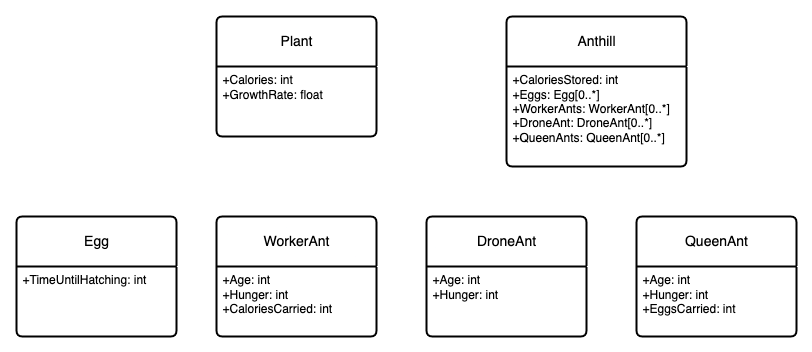
\includegraphics[scale=0.5]{entity_diagrams.png}


\section{Repository}
\url{https://github.com/alecwalsh/ant_colony_simulation}

\section{Bibliography}

\bibliography{sources}
\bibliographystyle{ieeetr}

\end{document}
